\externaldocument{methods}
\externaldocument{results}


\begin{figure}
\centering
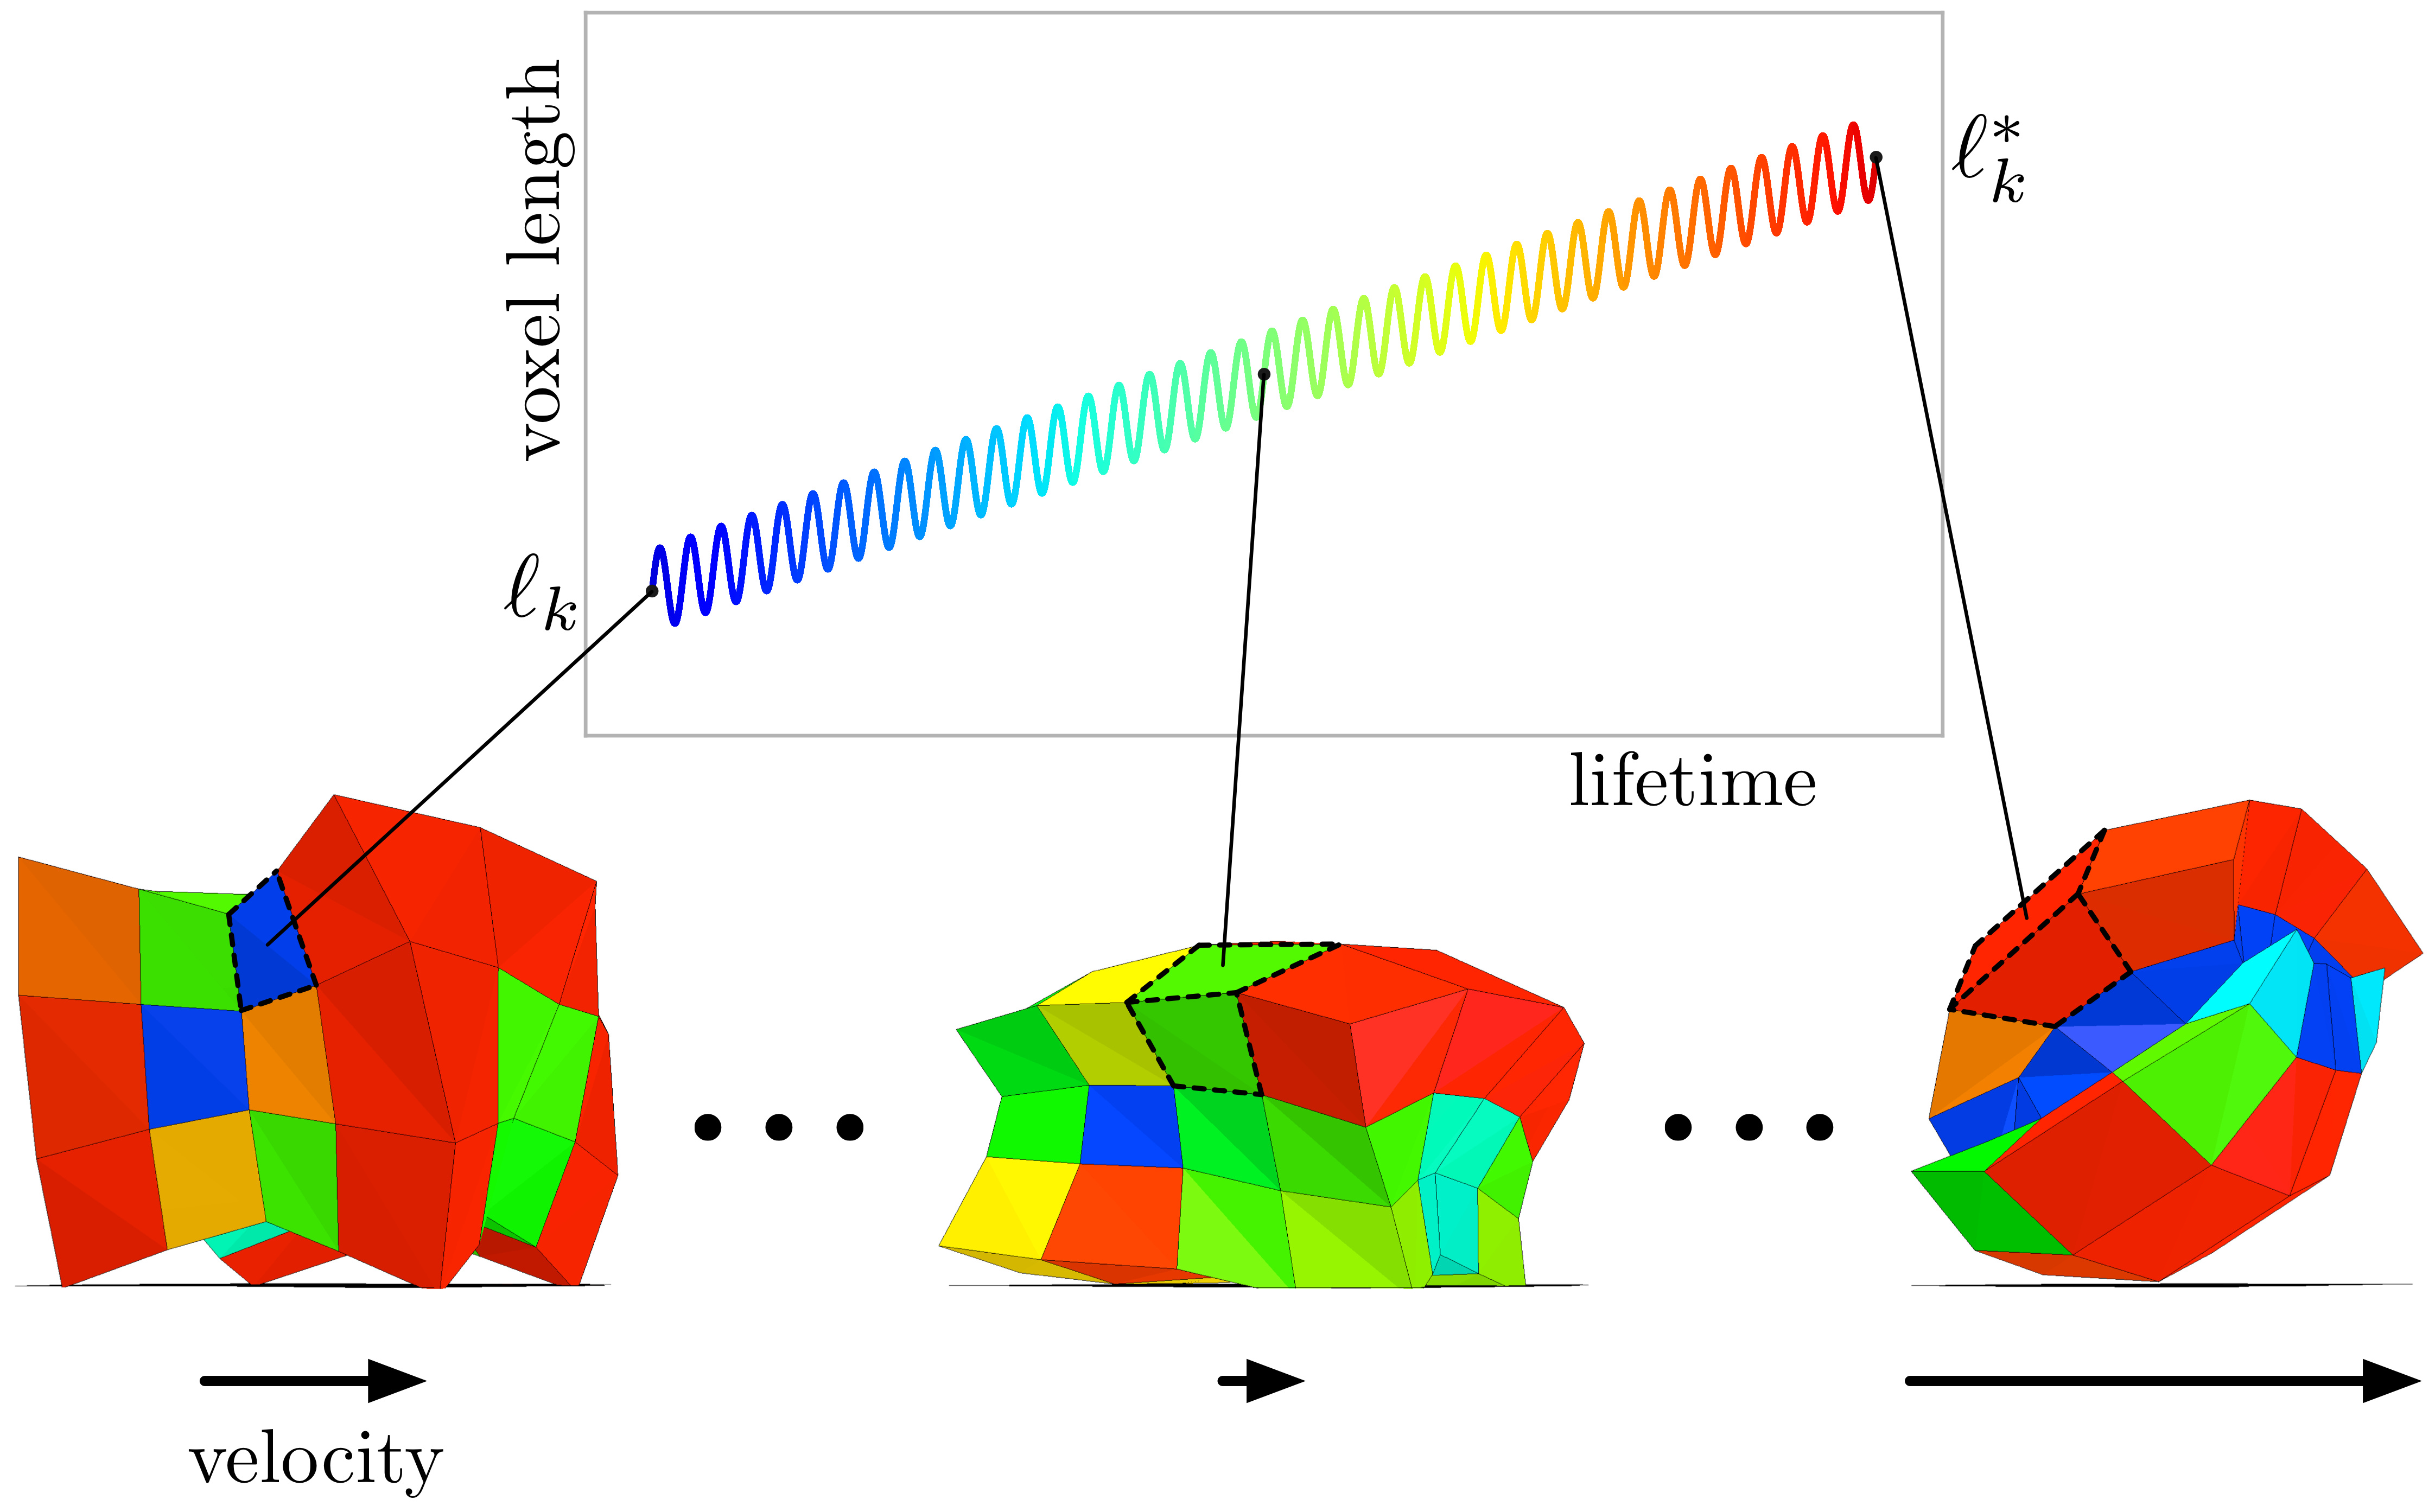
\includegraphics[width=0.8\linewidth]{Fig1}
\caption{\label{fig:blueprint}\textbf{Modeling development.} An evolved soft robot changes its shape during its lifetime (postnatal development), from a walking quadruped into a rolling form. 
Evolution dictates how a robot's morphology develops by setting each voxel's initial ($\ell_k$) and final ($\ell^*_k$) resting length.
The length of a single voxel $k$ is plotted to illustrate its (slower) growth and (faster) actuation processes.
Voxel color indicates the current length of that cell: the smallest voxels are blue, medium sized voxels are green, and the largest voxels are red.
As robots develop and interact with a physically realistic environment, they generate heterogeneous behavior in terms of instantaneous velocity (bottom arrows).
Soft robot evolution, development and physiological functioning can be seen in Supplementary \href{https://youtu.be/Ee2sU-AZWC4}{Video S1}.
}
\end{figure}

\begin{figure}
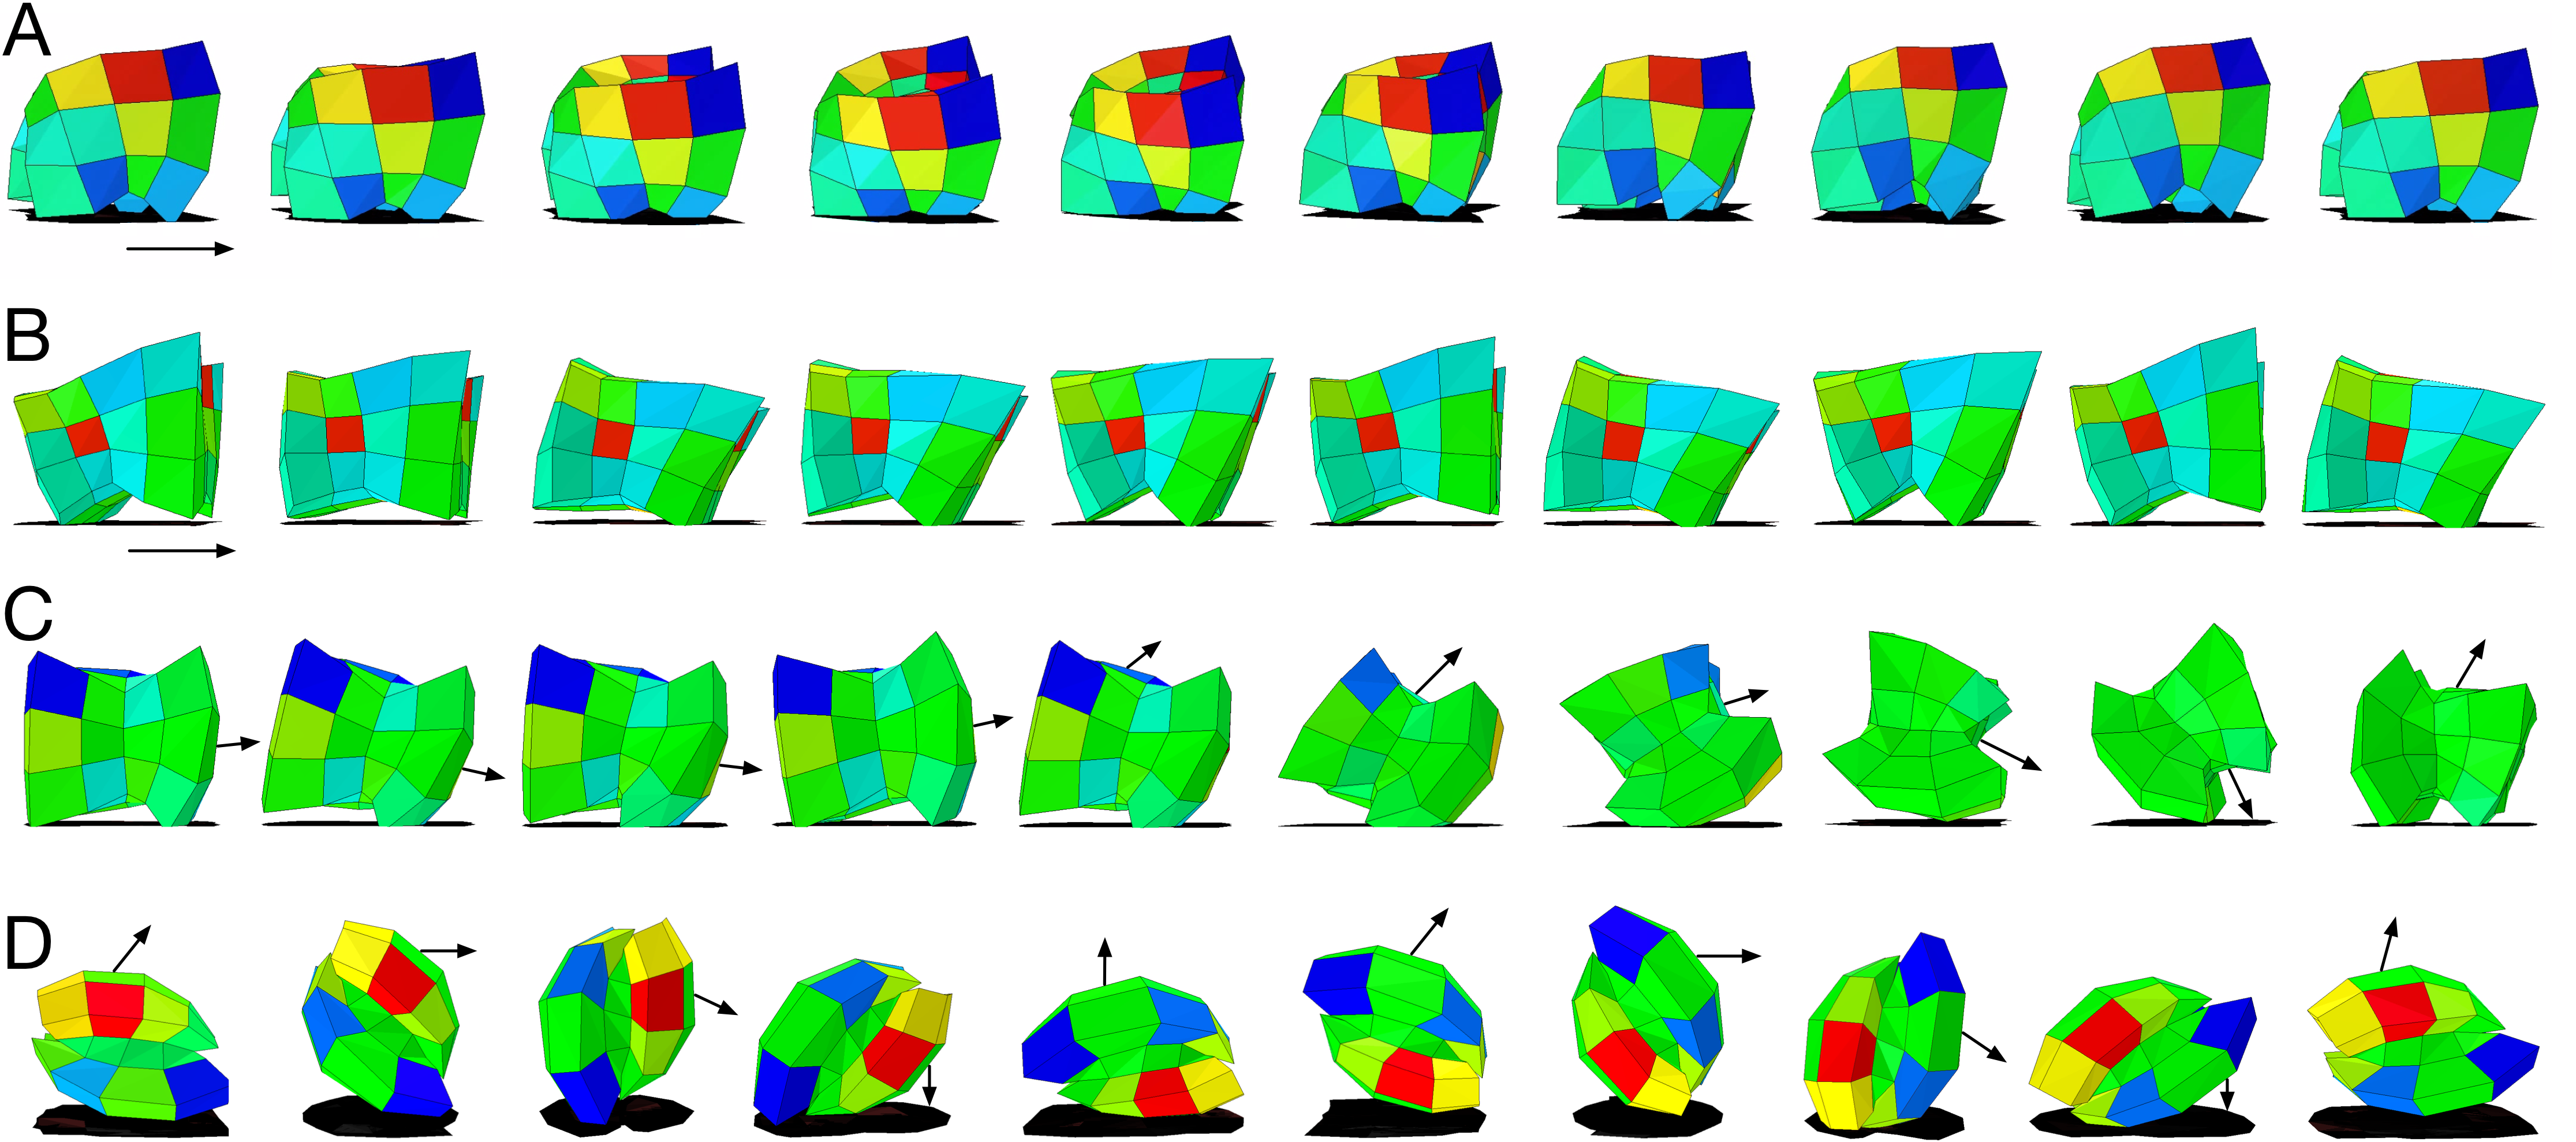
\includegraphics[width=\linewidth]{Fig2}
\caption{\label{fig:trot-gallop-roll}\textbf{Evolved behavior.}
Each row depicts a different evolved robot moving from left to right. 
Voxels in this figure are colored by the amount of subsequent morphological development remaining at that cell: blue indicates shrinking voxels $(\ell_k > \ell_k^*)$, red indicates growing voxels $(\ell_k < \ell_k^*)$, green indicates little to no change either way $(\ell_k \cong \ell_k^*)$.
(A) An evolved trotting soft quadruped with a two-beat gait synchronizing diagonal pairs of legs. 
(B) A galloping adult robot which goes fully airborne mid-gait.
(C) A galloping juvenile robot which develops into a rolling adult form. 
(D) A rolling juvenile robot at 10 points in ontogeny immediately after birth.
Arrows indicate the general directionality of movement,  
but this is more precisely captured by
Supplementary Video S1. 
}
\end{figure}

\begin{figure}
\centering
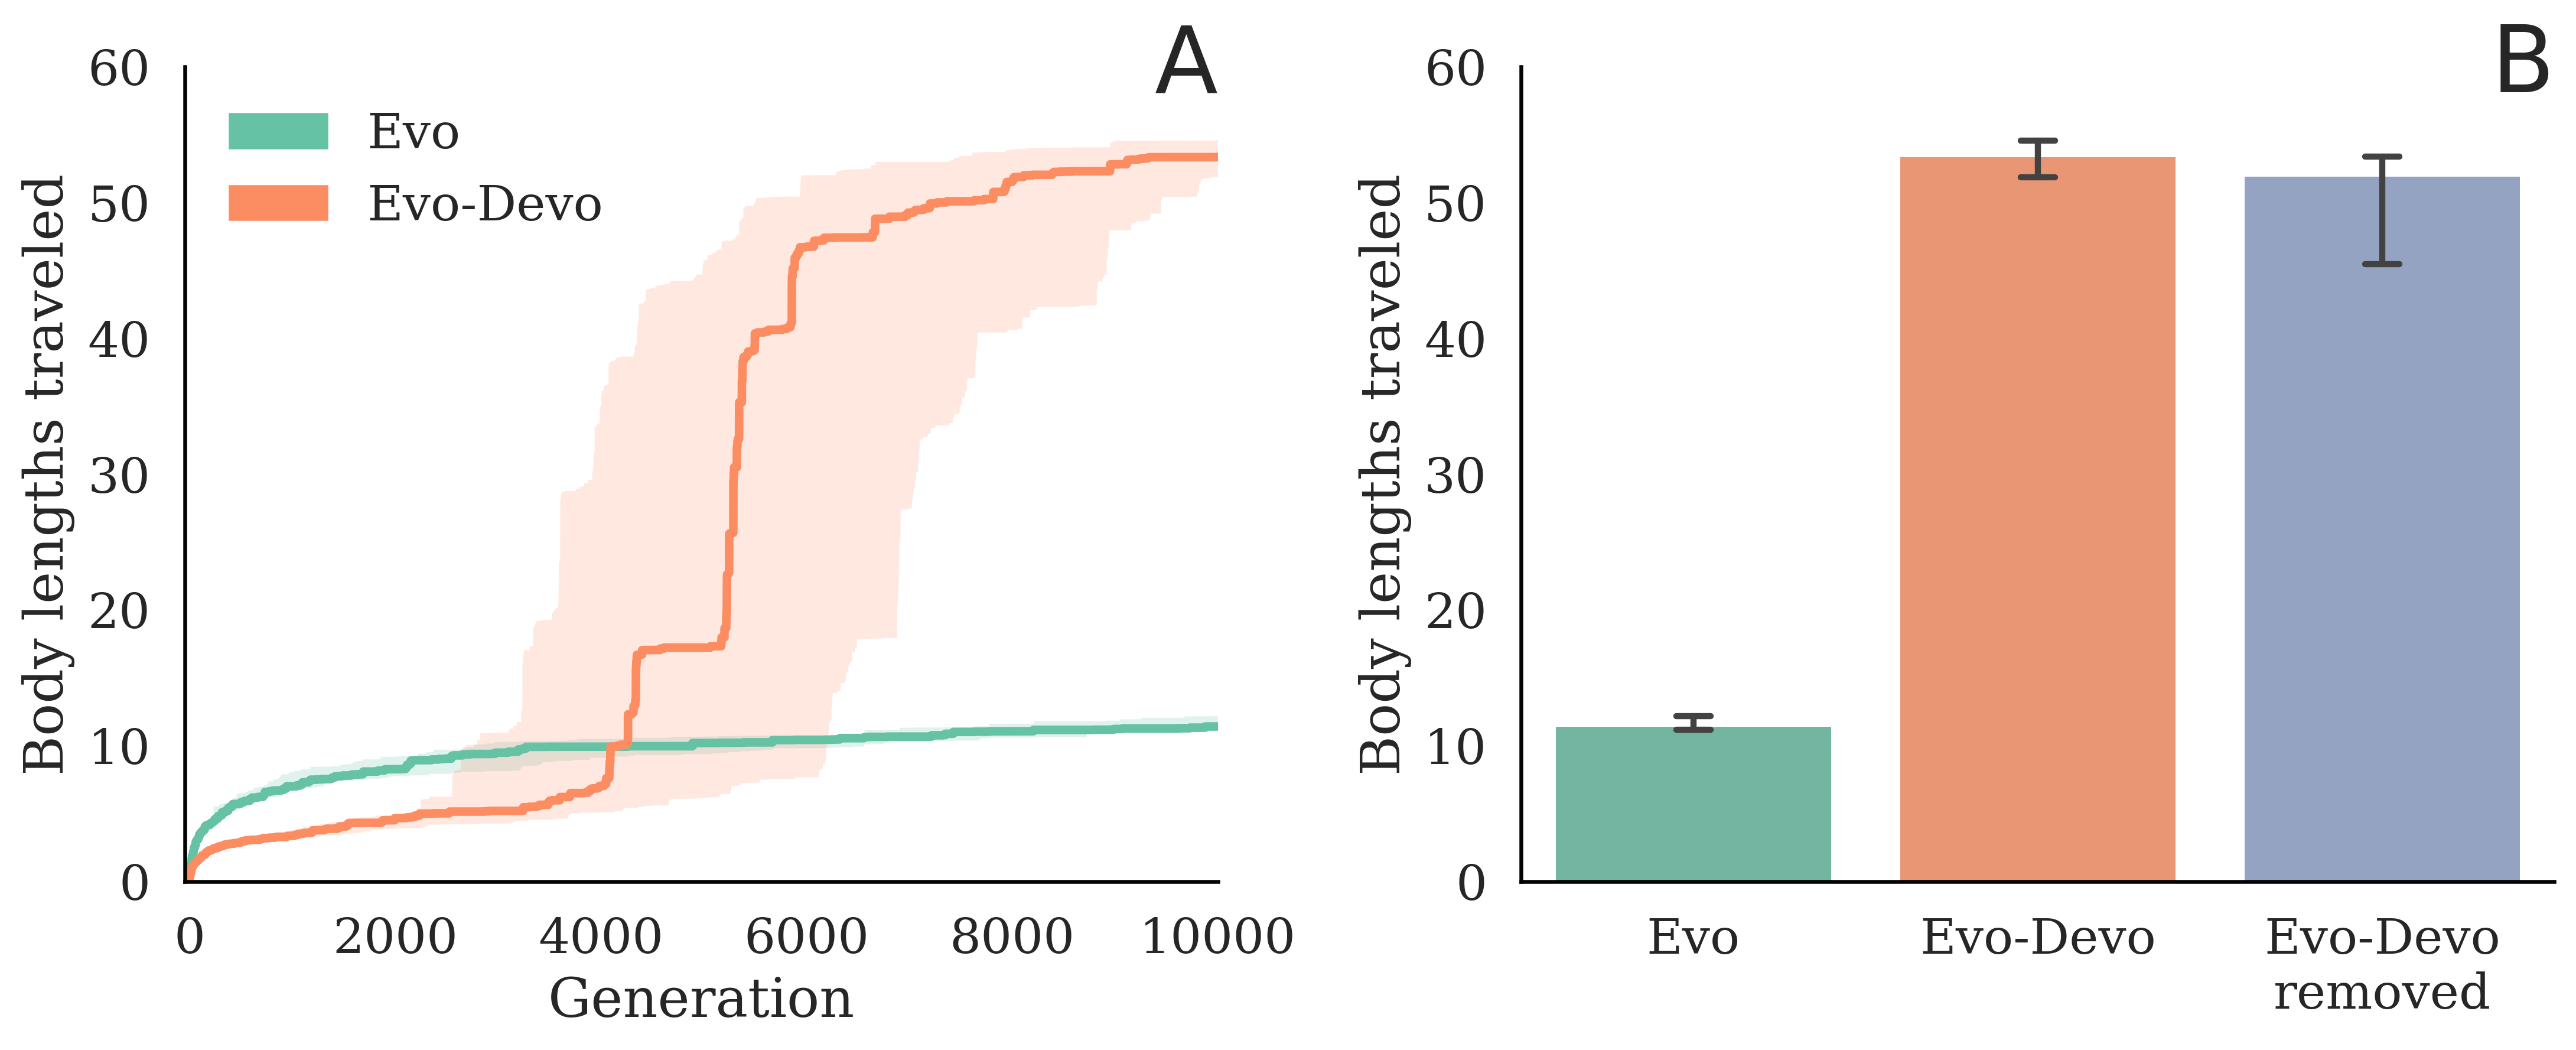
\includegraphics[width=0.9\linewidth]{Fig3}
\caption{\label{fig-fitness}\textbf{Evolvability and development.} Morphological development drastically increases evolvability (A), even when development is manually removed from the evolved systems (the run champions) by setting the final parameter values equal to their starting values ($\ell_k^*=\ell_k$ and $\phi_k^*=\phi_k$), in each voxel (B).
Median fitness is plotted with 95\% bootstrapped confidence intervals for three treatments: evolving but non-developmental robots (Evo), evolving and developing robots (Evo-Devo), and evolving and developing robots evaluated at the end of evolution with their development removed (Evo-Devo removed).
Fitness of just the final, evolved populations are plotted in B.}
\end{figure}

\begin{figure}
\centering
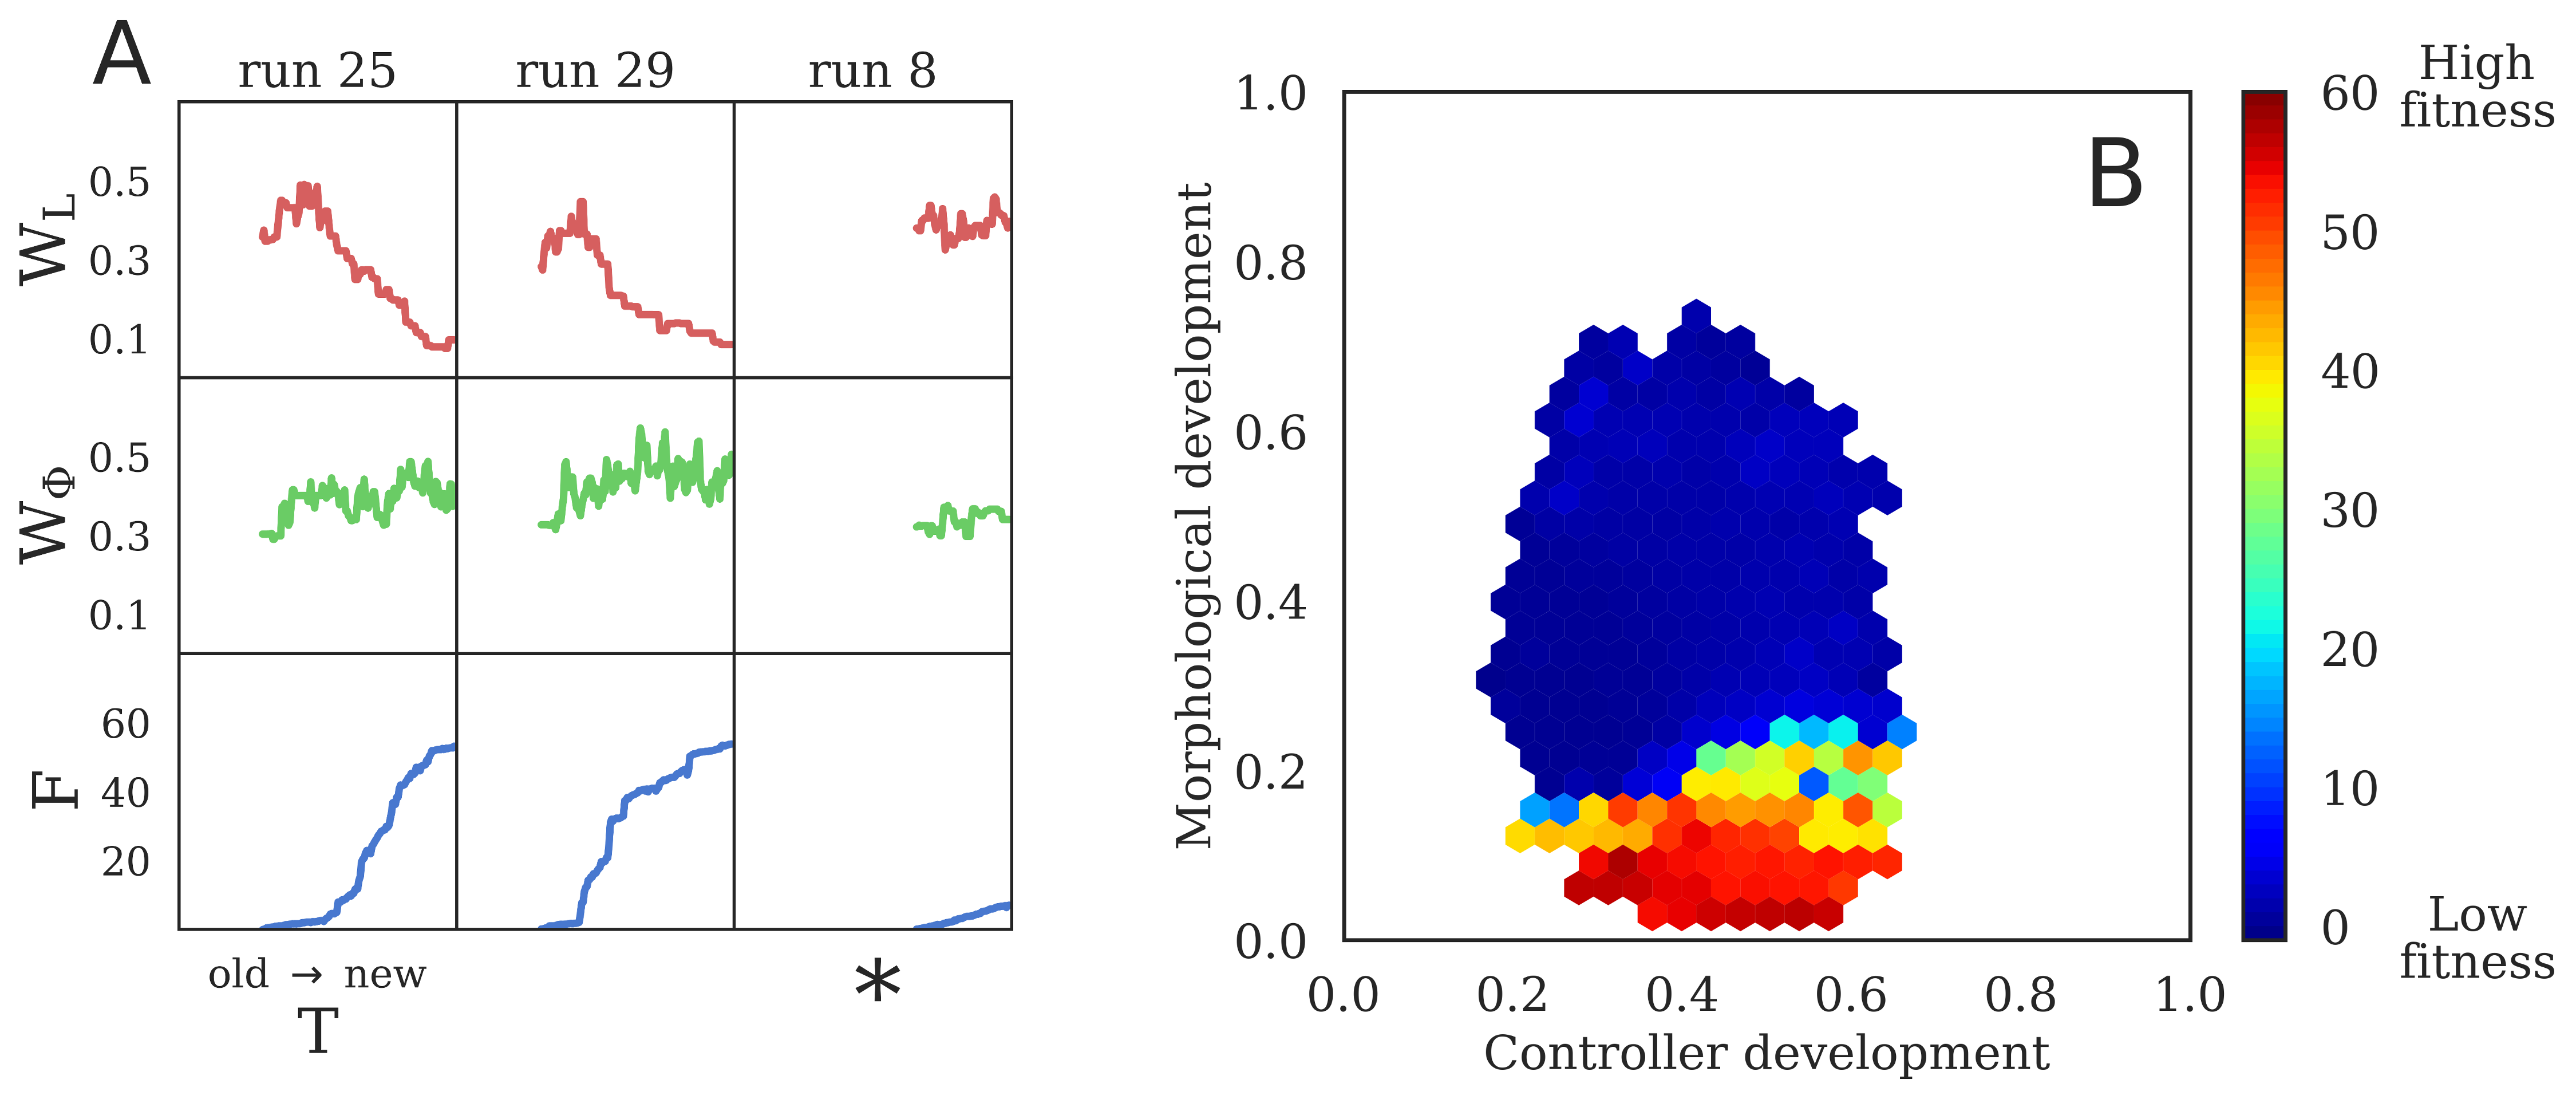
\includegraphics[width=\linewidth]{Fig4}
\caption{\label{fig-correlation}\textbf{Differential canalization.} 
Developmental windows (i.e.~the total lifetime developmental change) for morphology, $W_L$ (see Equation \ref{eq-WL}), and controller, $W_{\Phi}$ (see Equation \ref{eq-WPhi}), alongside fitness $F$.
(A) Three representative lineages taken from Supplementary Fig. S1, which displays the lineages of all 30 Evo-Devo run champions. Evolutionary time $T$ moves from the oldest ancestor (left) to the run champion (right). A general trend emerges wherein lineages initially increase their morphological development in $T$ (rising red curves) and subsequently decrease morphological development to almost zero (falling red curves). Five of the 30 evolutionary trials, annotated by {\Large $\ast$}, fell into a local optima.
(B) Median fitness as a function of morphology and controller development windows $(W_L,\; W_{\Phi})$, for all Evo-Devo designs evaluated. 
Overall, the fastest designs tend to have small amounts of morphological development, but are free to explore alternative control policies.}
\end{figure}

\begin{figure}
\centering
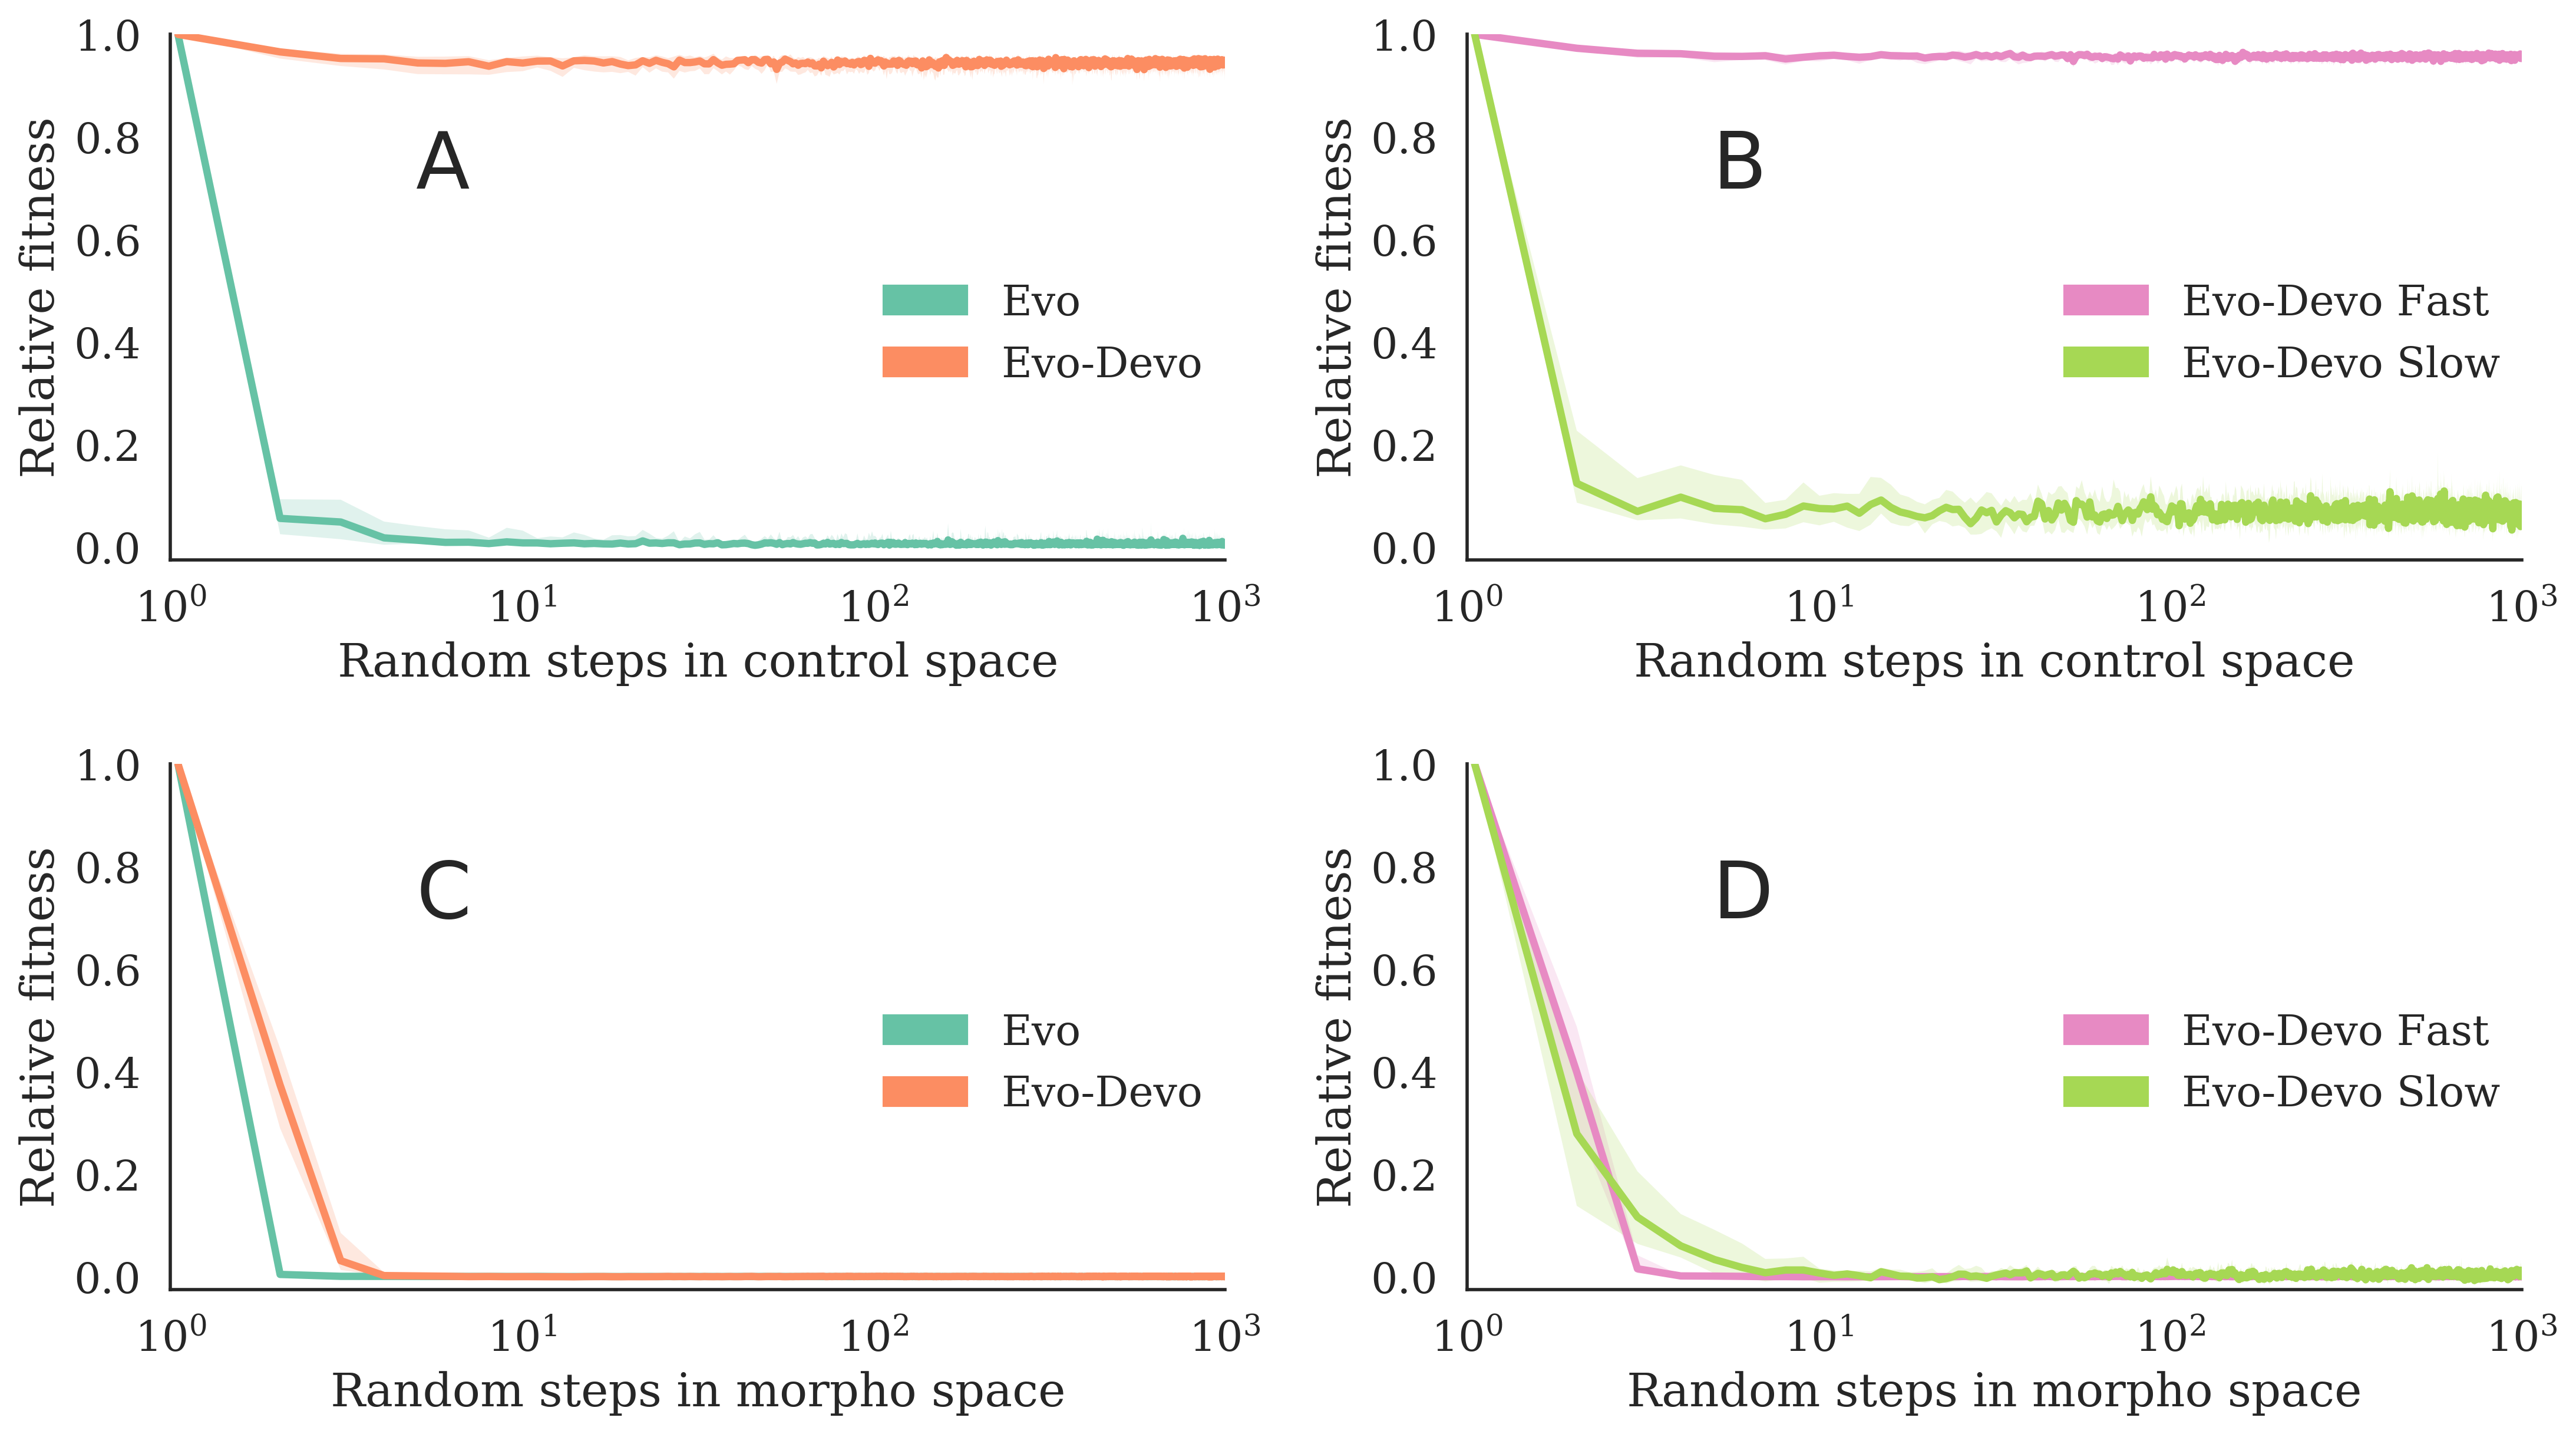
\includegraphics[width=\linewidth]{Fig5}
\caption{\label{fig-random-walks}\textbf{Sensitivity to morphological and control mutations.}
Ten random walks were taken from each run champion.
(A) Successive \textit{control} mutations to the Evo and Evo-Devo run champions.
(B) The previous Evo-Devo results separately for fast and slow design types.
(C) Successive \textit{morphological} mutations to the Evo and Evo-Devo run champions.
(D) The previous Evo-Devo results separately for fast and slow design types. Medians plotted with 99\% confidence intervals.
The faster Evo-Devo robots tend to possess body plans that are robust to control mutations.}
\end{figure}

\begin{figure}
\centering
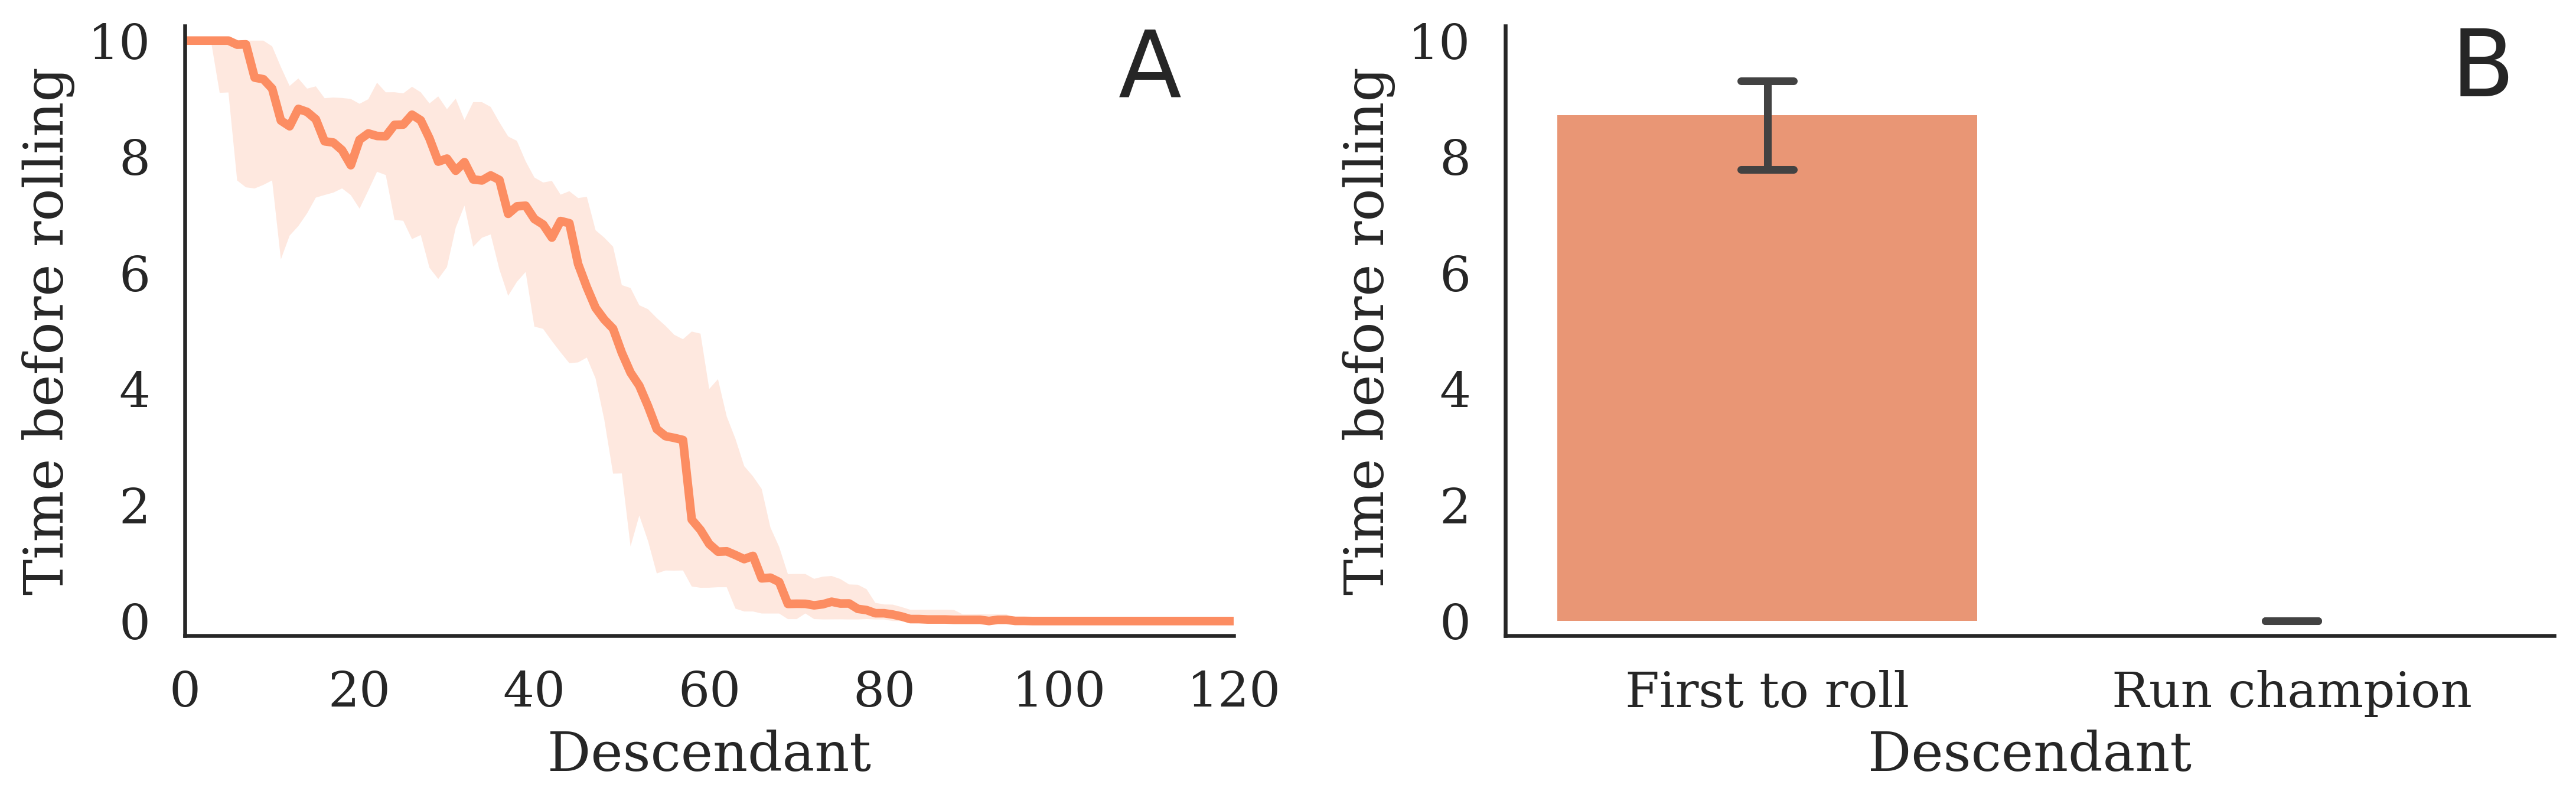
\includegraphics[width=0.9\linewidth]{Fig6}
\caption{\label{fig-discovery}\textbf{Late onset discoveries.} Ontogenetic time before the discovery of rolling over, taken from the lineages of the best robot from the each of the 25 Evo-Devo trials that produced a rolling design. Median time to discovery, with 95\% C.I.s, for (A) the lineage from the most distant ancestor $(T=0)$ to more recent descendants, and (B) the first ancestor to roll over compared to the final run champion. 
Rolling over is measured from the first time step the top of the robot touches the ground, rather than after completely rolling over. 
The first ancestors to roll over tend to do so at the end of their lives, their descendants tend to roll sooner in life, and the final run champions all begin rolling immediately at birth. 
These results are a consequence of dependent time steps: 
because mutational changes affect all downstream steps, their phenotypic impact is amplified in all but the terminal stages of development. Thus, late onset changes can provide exploration in the search space without breaking rest-of-life functionality, and subsequent evolution can gradually assimilate this trait to the start of development.}
\end{figure}

